\addcontentsline{toc}{chapter}{Занятие 1. Выборочные характеристики}
\chapter*{Занятие 1. Выборочные характеристики}

\addcontentsline{toc}{section}{Контрольные вопросы и задания}
\section*{Контрольные вопросы и задания}

\subsubsection*{Приведите определение выборки, вариационого ряда, статистики, порядковой статистики,
                эмпирической функции распределения.}

$x_1, \dotsc, x_n$ --- наблюдаемые значения ---
независимые одинаково распределённые случайные величины с неизвестной функцией распределения
$F \left( x \right) $.

Такой набор случайных величин называется выборкой из распределения $F$.

Вариационный ряд --- последовательность $x_{ \left( 1 \right) }, \dotsc, x_{ \left( n \right) }$,
полученная в результате расположения в порядке неубывания исходной последовательности
независимых одинаково распределённых случайных величин $x_1, \dotsc, x_n$.

Статистикой называют функцию $S$ от выборки $X = \left( x_1, x_2, \dotsc, x_n \right) $ такую,
что $S \left( X \right) = S \left( x_1, x_2, \dotsc, x_n \right) $.

Вариационный ряд и его члены являются порядковыми статистиками.

Эмпирической (выборочной) функцией распределения,
построенной по выборке $x_1, \dotsc, x_n$ называется функция
$$F_n \left( x \right) =
  \frac{1}{n} \sum \limits_{k = 1}^n \mathbbm{1}_{x_k \leq x}, \,
  x \in \mathbb{R}.$$

\subsubsection*{Какими свойствами обладает эмпирическая функция распределения?}

Есть множество полной вероятности,
на котором эмпирическая функция распределения аппроксимирует функцию распределения,
то есть почти наверное $F_n \Rightarrow F, \, n \to \infty $.

\subsubsection*{Запишите выражения для выборочного среднего, выборочной диспресии,
                выборочных моментов.}

$$ \frac{1}{n} \sum \limits_{k = 1}^n x_k$$
--- выборочное среднее.

Выборочная дисперсия
$$ \hat{ \sigma^2} =
  \frac{1}{n - 1} \sum \limits_{k = 1}^n \left( x_k - \overline{x} \right)^2.$$

Выборочные моменты в математической статистике ---
это оценка теоретических моментов распределения на основе выборки.

Выборочный момент порядка $k$ --- это случайная величина
$$a_n \left( k \right) =
   \frac{1}{n} \sum \limits_{i = 1}^n x_i^k.$$

\addcontentsline{toc}{section}{Аудиторные задачи}
\section*{Аудиторные задачи}

\subsubsection*{1.4}

\textit{Задание.}
Пусть $X_1, \dotsc, X_n$ ---
выборка из равномерного распределения на отрезке $ \left[0, \theta \right] $
с неизвестным параметром $ \theta $.
Какие из приведённых ниже функций являются статистиками?
\begin{enumerate}[label=\alph*)]
  \item $ \overline{X}$;
  \item $5X_{ \left( n \right) }$;
  \item $ \theta / 2$;
  \item $X_1 / \theta $;
  \item $X_{ \left( 1 \right) } + X_1 + X_n$.
\end{enumerate}

\textit{Решение.}
\begin{enumerate}[label=\alph*)]
  \item Да;
  \item да;
  \item нет, так как не функция от выборки;
  \item функция не только от выборки (зависит от неизвестного параметра).
  Отсюда следует, что это не статистика;
  \item да.
\end{enumerate}

\subsubsection*{1.5}

\textit{Задание.}
Пусть $X_1, \dotsc, X_n$ --- выборка из распределения Пуассона с параметром $ \lambda $.
Вычислите математическое ожидание и дисперсию статистики
$$ \overline{X} =
  \frac{1}{n} \sum \limits_{i = 1}^n X_i.$$
Выясните, имеет ли статистика $ \overline{X}$ распределение Пуассона.

\textit{Решение.} Все $X_i$ одинаково распределены.
Отсюда следует, что все математические ожидания одинаковы
$$M \overline{X} =
  \frac{1}{n} \sum \limits_{i = 1}^n MX_i =
  \frac{1}{n} \cdot nMX_1 =
  MX_1 =
  \lambda.$$

Для всякой выборки справедливо $M \overline{X} = MX_1$.

Из независимости $X_i$ получаем
$$D \overline{X} =
  \frac{1}{n^2} \sum \limits_{i = 1}^n DX_i.$$

Так как $X_i$ одинаково распределены, то все дисперсии одинаковы
$$D \overline{X} =
  \frac{DX_1}{n} =
  \frac{ \lambda }{n}.$$

Математическое ожидание и дисперсия для распределения Пуассона совпадают.
Отсюда следует, что эта случайная величина не имеет распределения Пуассона.

$ \overline{X}$ не обязательно буде принимать целые значения.

\subsubsection*{1.6}

\textit{Задание.} Вычислите математическое ожидание статистик:
\begin{enumerate}[label=\alph*)]
  \item $S^2 = \overline{X^2} - \left( \overline{X} \right)^2$;
  \item $S_0^2 =
          1 / \left( n - 1 \right) \cdot
          \sum \limits_{i = 1}^n \left( X_i - \overline{X} \right)^2$.
\end{enumerate}

\textit{Решение.}
\begin{enumerate}[label=\alph*)]
  \item Распишем каждую из величин
  $$S^2 =
    \overline{X^2} - \left( \overline{X} \right)^2 =
    \frac{1}{n} \sum \limits_{i = 1}^n X_i^2 -
    \left( \frac{1}{n} \sum \limits_{i = 1}^n X_i \right)^2.$$
  Распишем квадрат
  $$ \frac{1}{n} \sum \limits_{i = 1}^n X_i^2 -
    \left( \frac{1}{n} \sum \limits_{i = 1}^n X_i \right)^2
    \frac{1}{n} \sum \limits_{i = 1}^n X_i^2 -
    \frac{1}{n^2} \left(
      \sum \limits_{i = 1}^n X_i^2 + 2 \sum \limits_{i, j = 1, i < j}^n X_i X_j
    \right).$$
  Берём слева и справа математическое ожидание.
  Из того, что случайные величины в выборке одинаково распределены
  $$MS^2 =
    MX_1^2 - \frac{1}{n^2} \left[ nMX_1 + 2C_n^2 \left( MX_1 \right)^2 \right].$$
  Подставляем $C_n^2$ и группируем
  $$MX_1^2 - \frac{1}{n^2} \left[ nMX_1 + 2C_n^2 \left( MX_1 \right)^2 \right] =
    \frac{n - 1}{n} \cdot MX_1^2 - \frac{n - 1}{n} \left( MX_1 \right)^2.$$
  Вынесем общий множитель за скобки
  $$ \frac{n - 1}{n} \cdot MX_1^2 - \frac{n - 1}{n} \left( MX_1 \right)^2 =
    \frac{n - 1}{n} \left[ MX_1^2 - \left( MX_1 \right)^2 \right] =
    \frac{n - 1}{n} \cdot SX_1.$$
  Эта оценка смещена ассимптотически;
  \item выразим $S_0$ через $S$.
  Раскроем квадрат
  $$S_0^2 =
    \frac{1}{n - 1} \sum \limits_{i = 1}^n \left( X_i - \overline{X} \right)^2 =
    \frac{1}{n - 1}
    \sum \limits_{i = 1}^n \left( X_i^2 - 2X_i \overline{X} + \overline{X}^2 \right).$$
  Имеем сумму $n$ одинаковых слагаемых
  $$ S_0^2 =
    \frac{1}{n - 1}
    \left( n \overline{X^2} - 2 \left( \overline{X} \right)^2 n + n \overline{X}^2 \right) =
    \frac{n}{n - 1} \left[ \overline{X^2} - \left( \overline{X} \right)^2 \right] =
    \frac{n - 1}{n} \cdot S^2.$$
  Отсюда следует, что
  $$MS_0^2 =
    \frac{n}{n - 1} \cdot \frac{n - 1}{n} \cdot DX_1 =
    DX_1.$$
\end{enumerate}

\subsubsection*{1.7}

\textit{Задание.} Найдите в терминах функции распределения $F$ выборки $X_1, \dotsc, X_n$:
\begin{enumerate}[label=\alph*)]
  \item распределение $k$-ой порядковой статистики $X_{ \left( k \right) }$;
  \item вероятность
  $P \left( X_{ \left( k \right) } < y, \, X_{ \left( k + 1 \right) } \geq y \right) $.
\end{enumerate}

\textit{Решение.}
\begin{enumerate}[label=\alph*)]
  \item Сделали упорядочивание случайных величин
  $$X_{ \left( 1 \right) } \leq
    X_{ \left( 2 \right) } \leq
    \dotsc \leq
    X_{ \left( k \right) } \leq
    \dotsc \leq
    X_{ \left( n \right)}.$$

  По определению
  $F_{X_{ \left( k \right) }} \left( y \right) =
    P \left( X_{ \left( k \right) } \leq y \right) =
    P$\{хотя бы $k$ элементов выборки не превышает $y$\} =
  $$= \sum \limits_{i = k}^n P(A_i),$$
  где $A_i =$ \{ровно $i$ элементов выборки не превышают $y$\}.

  Есть $n$ испытаний, успех --- $X_i \leq y$.

  Вероятность успеха --- это $F \left( y \right) $, вероятность неудачи ---
  это $ \left[ 1 - F \left( y \right) \right] $.
  Это биномиальное распределение
  $$F_{X_{ \left( k \right) }} =
    \sum \limits_{i = k}^n
      C_n^i F^i \left( y \right) \left[ 1 - F \left( y \right) \right]^{n - i};$$
  \item согласно с предыдущим пунктом
  $P \left( X_{ \left( k \right) } < y, \, X_{ \left( k + 1 \right) } \geq y \right) =
    P$\{ровно $i$ элементов выборки не превышает $y$\} $=
    C_n^k F^k \left( y \right) \left[ 1 - F \left( y \right) \right]^{n - k}$.
\end{enumerate}

\subsubsection*{1.8}

\textit{Задание.}
Пусть $ \left( -0.8; 2.9; 4.5; -5.7; 1.1; -3.2 \right) $ --- наблюдаемые значения выборки.
Составьте вариационный ряд,
постройте эмпирическую функцию распределения $F_6 \left( x \right) $ и её график.
Вычислите выборочное среднее и выборочную дисперсию.

\textit{Решение.} Вариационный ряд: $ \left( -5.7; -3.2; -0.8; 1.1; 2.9; 4.3 \right) $.

Эмпирическая функция распределения (рис. \ref{fig:18}).
$$F_6 \left( y \right) =
  \frac{1}{6} \sum \limits_{i = 1}^6 \mathbbm{1} \left\{ x_i \leq y \right\} =
  \begin{cases}
    0, \qquad x < -5.7; \\
    \frac{1}{6}, \qquad -5.7 \leq x < -3.2, \\
    \frac{2}{6}, \qquad -3.2 \leq x < -0.8, \\
    \frac{3}{6}, \qquad -0.8 \leq x < 1.1, \\
    \frac{4}{6}, \qquad 1.1 \leq x < 2.9, \\
    \frac{5}{6}, \qquad 2.9 \leq x < 4.3, \\
    1, \qquad x \geq 4.3.
  \end{cases}$$

\begin{figure}[h!]
  \centering
  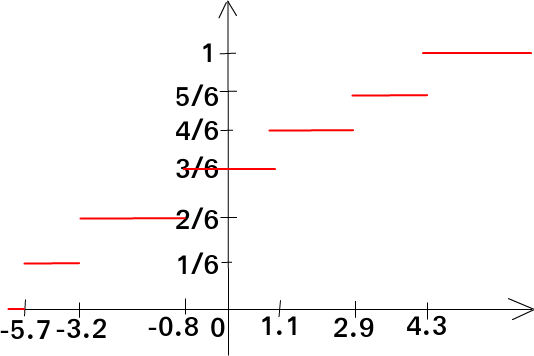
\includegraphics[width=.4\textwidth]{./pictures/1_8.png}
  \caption{Эмпирическая функция распределения}
  \label{fig:18}
\end{figure}

Выборочное среднее
$$ \overline{X} =
  \frac{1}{6} \left( -5.7 -3.2 - 0.8 + 1.1 + 2.9 + 4.3 \right) =
  \frac{1}{6} \left( -9.7 + 8.3 \right) =
  - \frac{1}{6} \cdot 1.4 =
  -0.23.$$

Выборочная дисперсия
$$ \hat{ \sigma }^2 =
  \frac{1}{5} \sum \limits_{i = 1}^6 \left( X_i + 0.23 \right)^2.$$
Она является несмещённой.

\subsubsection*{1.9}

\textit{Задание.}
Вычислите вероятность $P \left( F_n \left( y \right) < F_n \left( z \right) \right) $.

\textit{Решение.}
\begin{enumerate}[label=\alph*)]
  \item $y \geq z$.
  Событие невозможное, потому что $F_n \left( y \right) \geq F_n \left( z \right) $;
  \item рассмотрим случай, когда $y < z$.

  Тогда искомая вероятность равна
  $P \left( F_n \left( y \right) < F_n \left( z \right) \right) = P$
  \{в $ \left( y, z \right) $ попал хотя бы 1 элемент выборки\}
  $= 1 - P$\{в $ \left( y, z \right) $ ни один элемент выборки не попал\}.
  Случайные величины одинаково распределены,
  поэтому $1 - P$\{в $ \left( y, z \right) $ ни один элемент выборки не попал\} $= \\
  = \left[ 1 - P \left\{ x_i \notin \left( y, z \right) \right\} \right]^n =
  1 - \left[ 1 - P \left\{ x_1 \in \left( y, z \right) \right\} \right]^n = \\
  = 1 - \left[ 1 - P \left( x_1 < z \right) + P \left( x_1 < y \right) \right]^n =
  1 - \left[ 1 - F \left( z \right) + F \left( y \right) \right]^n$.
\end{enumerate}

\subsubsection{1.10}

\textit{Задание.} Пусть $X1, \dotsc, X_n$ --- выборка из распределения $F$ с плотностью $f$.
Найдите совместную плотность распределения всех порядковых статистик,
то есть плотность распределения случайного вектора
$ \left( X_{ \left( 1 \right) }, \dotsc, X_{ \left( n \right) } \right) $.

\textit{Решение.}
$F_{ \left( X_{ \left( 1 \right) }, X_{ \left( 2 \right) } \right) } \left( y_1, y_2 \right) =
  P \left( X_{ \left( 1 \right) } \leq y_1, \, X_{ \left( 2 \right) } \leq y_2 \right)$.
Воспользуемся формулой
$P \left( A \cap B \right) =
  P \left( B \right) - P \left( \overline{A} \cap B \right) $.
Получим
$$P \left( X_{ \left( 1 \right) } \leq y_1, \, X_{ \left( 2 \right) } \leq y_2 \right) =
  P \left( X_{ \left( 1 \right) } \leq y_2 \right) -
  P \left( X_{ \left( 1 \right) } > y_1, \, X_{ \left( 2 \right) } \leq y_2 \right).$$
Среди $X_{ \left( 1 \right) }$ и $X_{ \left( 2 \right) }$ случайная величина
$X_{ \left( 2 \right) }$ является максимальной.
\begin{equation*}
  \begin{split}
    P \left( X_{ \left( 1 \right) } \leq y_2 \right) -
    P \left( X_{ \left( 1 \right) } > y_1, \, X_{ \left( 2 \right) } \leq y_2 \right) = \\
    = P \left( X_1 \leq y_2, \, X_2 \leq y_2 \right) -
    P \left( X_1 \in \left( y_1, y_2 \right], \, X_2 \in \left( y_1, y_2 \right] \right).
  \end{split}
\end{equation*}
Случайные величины $X_1, X_2$ --- независимые и одинаково распределённые
\begin{equation*}
  \begin{split}
    P \left( X_1 \leq y_2, \, X_2 \leq y_2 \right) -
    P \left( X_1 \in \left( y_1, y_2 \right], \, X_2 \in \left( y_1, y_2 \right] \right) = \\
    = \begin{cases}
      \left[ F \left( y_2 \right) \right]^2, \qquad y_1 \geq y_2, \\
      \left[ F \left( y_2 \right) \right]^2 -
      \left[ F \left( y_2 \right) - F \left( y_1 \right) \right]^2, \qquad y_1 < y_2.
    \end{cases}
\end{split}
\end{equation*}

Продифференцируем
\begin{equation*}
    f_{ \left( X_{ \left( 1 \right) }, X_{ \left( 2 \right) } \right) } \left( y_1, y_2 \right) =
    \begin{cases}
      0, \qquad y_1 \geq y_2, \\
      2f \left( y_1 \right) f \left( y_2 \right), \qquad y_1 < y_2.
    \end{cases}
\end{equation*}

Рассматриваем множество всех векторов,
которые имеют упорядоченные координаты
$ \Delta = \left\{ \vec{x} \in \mathbb{R}^n \; : \; z_1 < z_2 < \dotsc < z_n \right\}, \,
  \Gamma \subseteq \Delta $
--- произвольное подмножество.

$ \left( X_{ \left( 1 \right) }, \dotsc, X_{ \left( n \right) } \right) \in
  \Delta$.

Чтобы найти вероятность того, что данный вектор принадлежит $ \Gamma $,
должны проинтегрировать плотность этого вектора по этому множеству
$$P \left\{
    \left( X_{ \left( 1 \right) }, \dotsc, X_{ \left( n \right) } \right) \in \Gamma
  \right\} =
  \int \limits_{ \Gamma }
    f_{ \left( X_{ \left( 1 \right) }, \dotsc, X_{ \left( n \right) } \right) }
    \left( z_1, \dotsc, z_n \right)
  dz_1 \dotsc dz_n.$$

С другой стороны,
$$P \left\{
    \left( X_{ \left( 1 \right) }, \dotsc, X_{ \left( n \right) } \right) \in \Gamma
  \right\} =
  \sum \limits_{ \sigma \in S_n}
    P \left\{
      \left( X_{ \sigma \left( 1 \right) }, \dotsc, X_{ \sigma \left( n \right) } \right) \in \Gamma
    \right\}.$$
Учтём все перестановки
$$ \sum \limits_{ \sigma \in S_n}
  P \left\{
    \left( X_{ \sigma \left( 1 \right)}, \dotsc, X_{ \sigma \left( n \right) } \right) \in \Gamma
  \right\} =
  n! P \left\{ \left( X_1, \dotsc, X_n \right) \in \Gamma \right\}.$$
Подставим найденное выражение для вероятности
$$n! P \left\{ \left( X_1, \dotsc, X_n \right) \in \Gamma \right\}
  n! \cdot
  \int \limits_{ \Gamma }
    f \left( z_1 \right) \cdot \dotsc \cdot f \left( z_n \right)
  dz_1 \dotsc dz_n.$$

Сравниваем полученные выражения
$$f_{ \left( X_{ \left( 1 \right) }, \dotsc, X_{ \left( n \right) } \right) }
  \left( z_1, \dotsc, z_n \right) =
  n! f \left( z_1 \right) \cdot \dotsc \cdot f \left( z_n \right) \cdot
  \mathbbm{1} \left\{ z_1 < z_2 < \dotsc < z_n \right\}$$
--- плотность вектора упорядоченных статистик.

\subsubsection*{1.11}

\textit{Задание.}
Пусть задана выборка $X_1, \dotsc, X_n$ из показательного распределения с параметром $ \alpha $.
\begin{enumerate}[label=\alph*)]
  \item Докажите,
  что случайные величины
  $X_{ \left( 1 \right) },
    X_{ \left( 2 \right) } - X_{ \left( 1 \right) },
    \dotsc,
    X_{ \left( n \right) } - X_{ \left( n - 1 \right) }$
  являются независимыми;
  \item найдите распределение разности $X_{ \left( k + 1 \right) } - X_{ \left( k \right) }$
  соседних порядковых статистик.
\end{enumerate}

\textit{Решение.}
$ \vec{ \xi } = \left( \xi_1, \dotsc, \xi_n \right) $ ---
случайный вектор с плотностью распределения $f_{ \vec{ \xi }} \left( \vec{x} \right) $.

Линейное преобразование этого вектора $ \vec{ \eta } = A \vec{ \xi }$, где $A$ ---
некоторая $n$-мерная матрица.

$$f_{A \vec{ \xi }} \left( \vec{y} \right) =
  \frac{1}{ \left| detA \right| } \cdot f_{ \vec{ \xi }} \left( A^{-1} \vec{y} \right).$$

Составим вектор из величин
$X_{ \left( 1 \right) },
  X_{ \left( 2 \right) } - X_{ \left( 1 \right) },
  \dotsc,
  X_{ \left( n \right) } - X_{ \left( n - 1 \right) }$.
Его плотность должна распасться на произведение плотностей компонент.

Из задачи 1.10
$$f_{ \left( X_{ \left( 1 \right) }, \dotsc, X_{ \left( n \right) } \right) }
  \left( y_1, \dotsc, y_n \right) =
  n! f \left( y_1 \right) \cdot \dotsc \cdot f \left( y_n \right) \cdot
  \mathbbm{1} \left\{y_1 < y_2 < \dotsc < y_n \right\}.$$
Подставим плотность показательного распределения
\begin{equation*}
  \begin{split}
    n! f \left( y_1 \right) \cdot \dotsc \cdot f \left( y_n \right) \cdot
    \mathbbm{1} \left\{y_1 < y_2 < \dotsc < y_n \right\} = \\
    = n! \alpha e^{- \alpha y_1} \cdot \mathbbm{1} \left\{ y_1 > 0 \right\} \cdot \dotsc \cdot
    \alpha e^{- \alpha y_n} \cdot \mathbbm{1} \left\{ y_n > 0 \right\} \cdot
    \mathbbm{1} \left\{ y_1 < y_2 < \dotsc < y_n \right\}.
  \end{split}
\end{equation*}
Перемножим
\begin{equation*}
  \begin{split}
    n! \alpha e^{- \alpha y_1} \cdot \mathbbm{1} \left\{ y_1 > 0 \right\} \cdot \dotsc \cdot
    \alpha e^{- \alpha y_n} \cdot \mathbbm{1} \left\{ y_n > 0 \right\} \cdot
    \mathbbm{1} \left\{ y_1 < y_2 < \dotsc < y_n \right\} = \\
    = n! \alpha^n e^{- \alpha \left( y_1 + \dotsc + y_n \right) } \cdot
    \mathbbm{1} \left\{ 0 < y_1 < y_2 < \dotsc < y_n \right\}.
  \end{split}
\end{equation*}

Нужно найти линейное преобразование
$$\begin{bmatrix}
    X_{ \left( 1 \right) } \\
    X_{ \left( 2 \right) } - X_{ \left( 1 \right) } \\
    X_{ \left( 3 \right) } - X_{ \left( 2 \right) } \\
    \dotsc \\
    X_{ \left( n \right) } - X_{ \left( n - 1 \right) }
  \end{bmatrix} =
  \begin{bmatrix}
    1 & 0 & 0 & 9 & \dots & 0 & 0 & 0\\
    -1 & 1 & 0 & 9 & \dots & 0 & 0 & 0\\
    0 & -1 & 1 & 0 & \dotsc & 0 & 0 & 0\\
    \dotsc \\
    0 & 0 & 0 & 0 & \dotsc & 0 & -1 & 1
  \end{bmatrix}
  \begin{bmatrix}
    X_{ \left( 1 \right) )} \\
    X_{ \left( 2 \right) } \\
    X_{ \left( 3 \right) } \\
    \dotsc \\
    X_{ \left( n \right) }
  \end{bmatrix},$$
где
$$\begin{bmatrix}
    1 & 0 & 0 & 0 & \dots & 0 & 0 & 0\\
    -1 & 1 & 0 & 0 & \dots & 0 & 0 & 0\\
    0 & -1 & 1 & 0 & \dotsc & 0 & 0 & 0\\
    \dotsc \\
    0 & 0 & 0 & 0 & \dotsc & 0 & -1 & 1
  \end{bmatrix} =
  A.$$

Определитель $detA = 1$.

Ищем обратную матрицу
$$\begin{bmatrix}
    1 & 0 & 0 & 0 & \dots & 0 \\
    1 & 1 & 0 & 0 & \dots & 0 \\
    1 & 1 & 1 & 0 & \dotsc & 0 \\
    \dotsc \\
    1 & 1 & 1 & 1 & \dotsc & 1
  \end{bmatrix}
  \begin{bmatrix}
    X_{ \left( 1 \right) } \\
    X_{ \left( 2 \right) } - X_{ \left( 1 \right) } \\
    X_{ \left( 3 \right) } - X_{ \left( 2 \right) } \\
    \dotsc \\
    X_{ \left( n \right) } - X_{ \left( n - 1 \right) }
  \end{bmatrix} =
  \begin{bmatrix}
    X_{ \left( 1 \right) )} \\
    X_{ \left( 2 \right) } \\
    X_{ \left( 3 \right) } \\
    \dotsc \\
    X_{ \left( n \right) }
  \end{bmatrix}.$$

Тогда имеем выражение
$$A^{-1} \vec{y} =
  \begin{bmatrix}
    y_1 \\
    y_1 + y_2 \\
    \dotsc \\
    \sum \limits_{i = 1}^n y_i
  \end{bmatrix}.$$

Определим искомый вектор через
$$ \vec{ \eta } =
  \left(
    X_{ \left( 1 \right) },
    X_{ \left( 2 \right) } - X_{ \left( 1 \right) },
    \dotsc,
    X_{ \left(n \right) } - X_{ \left( n - 1 \right) }
  \right).$$
Тогда
\begin{equation*}
  \begin{split}
    f_{ \vec{ \eta }} \left( y_1, \dotsc, y_n \right) = \\
    = n! \alpha^n e^{- \alpha \left( ny_1 + \left( n - 1 \right) y_2 + \dotsc + y_n \right) } \cdot
    \mathbbm{1} \left\{ 0 < y_1 < y_1 + y_2 < \dotsc < y_1 + y_2 + \dotsc + y_n \right\}.
  \end{split}
\end{equation*}
Разобъём на $n$ множителей
\begin{equation*}
  \begin{split}
    n! \alpha^n e^{- \alpha \left( ny_1 + \left( n - 1 \right) y_2 + \dotsc + y_n \right) } \cdot
    \mathbbm{1} \left\{ 0 < y_1 < y_1 + y_2 < \dotsc < y_1 + y_2 + \dotsc + y_n \right\} = \\
    = \left[ n \alpha e^{- \alpha ny_1} \cdot \mathbbm{1} \left\{ 0 < y_1 \right\} \right] \cdot
    \left[
      \left( n - 1 \right) \alpha e^{- \alpha \left( n - 1 \right) y_2} \cdot
      \mathbbm{1} \left\{ y_2 > 0 \right\}
    \right] \cdot \dotsc \times \\
    \times \left[ \alpha e^{- \alpha y_n} \cdot \mathbbm{1} \left\{ y_n > 0 \right\} \right].
  \end{split}
\end{equation*}

Имеем произведение плотностей компонент, значит,
элементы вектора независимы и показательно распределены с параметром
$ \alpha \left( n - k \right) $,
то есть
$X_{ \left( k + 1 \right) } - X_{ \left( k \right) } \sim
  \Pi \left( \alpha \left( n - k \right) \right) $.
Считаем, что $X_{ \left( 0 \right) } = 0$.

\addcontentsline{toc}{section}{Домашнее задание}
\section*{Домашнее задание}

\subsubsection*{1.15}

\textit{Задание.}
Пусть $X_1, \dotsc, X_n$ ---
выборка из равномерного на отрезке $ \left[ a, b \right] $ распределения.
Вычислите математическое ожидание и дисперсию статистики
$$ \overline{X} =
  \frac{1}{n} \sum \limits_{i = 1}^n X_i.$$
Выясните, имеет ли статистика $ \overline{X}$ равномерное распределение; нормальное распределение.

\textit{Решение.} Все $X_i$ одинаково распределены.
Отсюда следует, что все математические ожидания одинаковы
$$M \overline{X} =
  \frac{1}{n} \sum \limits_{i = 1}^n MX_i =
  \frac{1}{n} \cdot nMX_1 =
  MX_1 =
  \frac{a+b}{2}.$$

Из независимости $X_i$ получаем
$$D \overline{X} =
  \frac{1}{n^2} \sum \limits_{i = 1}^n DX_i.$$

Так как $X_i$ одинаково распределены, то все дисперсии одинаковы
$$D \overline{X} =
  \frac{DX_1}{n} =
  \frac{ \left( b - a \right)^2}{12n}.$$

Чтобы выяснить,
распределена ли статистика $ \overline{X}$ по нормальному или равномерному распределению,
найдём её характеристическую функцию $ \varphi_{ \overline{X}} \left( t \right) $.
Учитывая независимость элементов выборки и то, что
$$ \varphi_{X_1} \left( t \right) =
  \dotsc =
  \varphi_{X_n} \left( t \right) =
  \frac{e^{itb} - e^{ita}}{it \left( b - a \right) },$$
находим
$$ \varphi_{ \overline{X}} \left( t \right) =
  \varphi_{X_1} \left( \frac{t}{n} \right) \cdot
  \dotsc \cdot
  \varphi_{X_n} \left( \frac{t}{n} \right) =
  \left[ \frac{\left( e^{itb} - e^{ita} \right) n}{it \left( b - a \right)} \right]^n.$$
Отсюда следует, что $ \overline{X}$ не имеет указанных распределений.

\subsubsection*{1.16}

\textit{Задание.}
Пусть $X_1, \dotsc, X_n$ --- выборка из некоторого распределения вероятностей,
функция распределения которого $F$ является непрерывной и строго возрастающей.
Найдите распределение выборки $Y_1, \dotsc, Y_n$, где
$$Y_i =
  F \left( X_i \right).$$

\textit{Решение.}
По определению
$$F_{ \eta_1, \dotsc, \eta_n} \left( X_1, \dotsc, X_n \right) =
  P \left( \eta_1 \leq X_1, \dotsc, \eta_n \leq X_n \right).$$
Воспользуемся независимостью
$$P \left( \eta_1 \leq X_1, \dotsc, \eta_n \leq X_n \right) =
  P \left( \eta_1 \leq X_1 \right) \cdot \dotsc \cdot P \left( \eta_n \leq X_n \right).$$

Функция распределения $i$-й компоненты вектора равна
$$F_{ \eta_i} \left( x \right) =
  P \left( F_{ \xi_i} \left( X_i \right) \leq x \right) =
  \begin{cases}
    0, \qquad x \leq 0, \\
    1, \qquad x > 1.
  \end{cases}$$

Рассмотрим $ \left[ 0, 1 \right] $.

Поскольку $F$ --- непрерывная и строго возрастающая, то существует $F^{-1} \left( x \right) $.
Обозначим через $z$ точку $F^{-1} \left( x \right) $ такую, что $F \left( z \right) = x$.
Событие $ \left\{ \eta = F \left( \xi \right) < x \right\} $ происходит тогда и только тогда,
когда происходит событие $ \left\{ \xi < z \right\} $.

Получаем на отрезке $ \left[ 0, 1 \right] $ равномерное распределение
$$F_{ \eta } \left( x \right) =
  F_{ \xi } \left( z \right) =
  F_{ \xi } \left( F_{ \xi }^{-1} \left( x \right) \right) =
  \begin{cases}
    0, \qquad x \leq 0, \\
    x, \qquad x \in \left( 0, 1 \right] ,\\
    1, \qquad x > 1.
  \end{cases}$$

\subsubsection*{1.17}

\textit{Задание.}
Пусть $X_1, \dotsc, X_n$ ---
выборка из дискретного распределения с вероятностями $P \left( X_1 = m \right) = p_m$, где
$$ \sum \limits_{m = 0}^N p_m =
  1.$$
Найдите распределение $k$-й порядковой статистики $X_{ \left( k \right) }$.

\textit{Решение.}
Сделали упорядочивание случайных величин
$$X_{ \left( 1 \right) } \leq
  X_{ \left( 2 \right) } \leq
  \dotsc \leq
  X_{ \left( k \right) } \leq
  \dotsc \leq
  X_{ \left( n \right)}.$$

По определению
$F_{X_{ \left( k \right) }} \left( y \right) =
  P \left( X_{ \left( k \right) } \leq y \right) =
  P$\{хотя бы $k$ элементов выборки не превышает $y$\} =
$$= \sum \limits_{i = k}^n P(A_i),$$
где $A_i =$ \{ровно $i$ элементов выборки не превышают $y$\}.

Есть $n$ испытаний, успех --- $X_i \leq y$.

Вероятность успеха --- это $F \left( y \right) $, вероятность неудачи ---
это $ \left[ 1 - F \left( y \right) \right] $.
Это биномиальное распределение
$$F_{X_{ \left( k \right) }} =
  \sum \limits_{i = k}^n
    C_n^i F^i \left( y \right) \left[ 1 - F \left( y \right) \right]^{n - i}.$$

Представим $F_{X_i} \left( y \right) = F \left( y \right) $ через $m$.
Запишем по определению
$$F_{X_1} \left( y \right) =
  P \left( X_1 \leq y \right) =
  \sum \limits_{m = 1}^n P \left( X_1 = m \right) =
  \sum \limits_{m = 1}^n p_m.$$

Подставим полученное выражение в функцию распределения
$$F_{X_{ \left( k \right) }} =
  \sum \limits_{i = k}^n
    C_n^i \sum \limits_{m = 1}^n p_m \left( 1 - \sum \limits_{m = 1}^n \right)^{n - i}.$$

\subsubsection*{1.18}

\textit{Задание.} Пусть $ \left( 3, 0, 4, 3, 6, 0, 3, 1 \right) $ --- наблюдаемые значения выборки.
Составьте вариационный ряд,
постройте эмпирическую функцию распределения $F_8 \left( x \right) $ и её график.
Вычислите выборочное среднее и выборочную дисперсию.

\textit{Решение.} Вариационный ряд: $ \left( 0, 0, 1, 3, 3, 3, 4, 6 \right) $.

Эмпирическая функция распределение (рис. \ref{fig:118})
$$F_8 \left( y \right) =
  \frac{1}{8} \sum \limits_{i = 1}^8 \mathbbm{1} \left\{ x_i \leq y \right\} =
  \begin{cases}
    0, \qquad x < 0, \\
    \frac{2}{8} = \frac{1}{4}, \qquad 0 \leq x < 1, \\
    \frac{3}{8}, \qquad 1 \leq x < 3, \\
    \frac{6}{8} = \frac{3}{4}, \qquad 3 \leq x < 4, \\
    \frac{7}{8}, \qquad 4 \leq x < 6, \\
    1, \qquad x \geq 6.
  \end{cases}$$

\begin{figure}[h!]
  \centering
  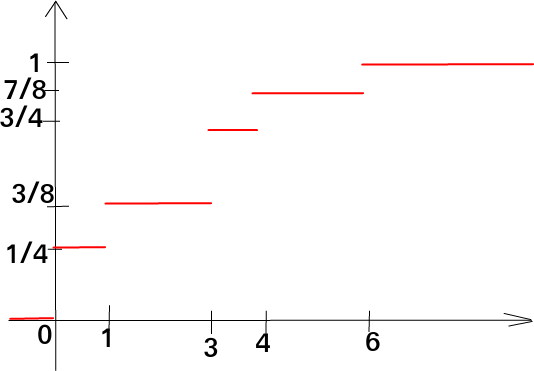
\includegraphics[width=.4\textwidth]{./pictures/1_18.png}
  \caption{Эмпирическая функция распределения}
  \label{fig:118}
\end{figure}

Выборочное среднее
$$ \overline{X} =
  \frac{1}{8} \left( 0 + 0 + 1 + 3 + 3 + 4 + 6 \right) =
  \frac{1}{8} \cdot 20 =
  \frac{10}{4} =
  2.5.$$

Выборочная дисперсия
\begin{equation*}
\begin{split}
  \hat{ \sigma^2} =
  \frac{1}{7} \sum \limits_{i = 1}^8 \left( X_i - 2.5 \right)^2 = \\
  = \frac{1}{7}
  \left[
    2 \left( 0 - 2.5 \right)^2 +
    \left( 1 - 2.5 \right)^2 +
    3 \left( 3 - 2.5 \right)^2 +
    \left( 4 - 2.5 \right)^2 +
    \left( 6 - 2.5 \right)^2
  \right] = \\
  = \frac{1}{7} \left( 12.5 + 2.25 + 0.75 + 2.25 + 12.25 \right) =
  \frac{30}{7} \approx
  4.29.
\end{split}
\end{equation*}

\subsubsection*{1.19}

\textit{Задание.}
По выборке объёма $n$ из распределения Бернулли с параметром $p$
постройте эмпирическую функцию распределения $F_n \left( y \right) $.

\textit{Решение.}
Случайная величина имеет распределение Бернулли, если она принимает всего два значения:
1 и 0 с вероятностями $p$ и $ \left( 1 - p \right) $ соответственно.
Таким образом: $P \left( x = 1 \right) = p, \, P \left( x = 0 \right) = 1 - p$.

Эмпирической функцией распределения, построенной по выборке
$$x_1, \dotsc, x_n,$$
называется функция
$$F_n \left( y \right) =
  \frac{1}{n} \sum \limits_{k = 1}^n \mathbbm{1} \left( x_k \leq y \right).$$

Пускай есть набор из $n$ чисел (нулей и единиц) --- выборка из распределения Бернулли.

Для удобства выстроим числа в порядке их возрастания:
$$0, 0, \dotsc, 0, 1, 1, \dotsc, 1.$$

Видим, что слева от нуля эмпирическая функция распределения будет равна нулю.

В точке 0 произойдёт скачок на
$$ \frac{n - k}{n},$$
где $k$ --- количество единиц, а $ \left( n - k \right) $ --- количество нулей в выборке.

В точке 1 будет скачок на
$$1 - \frac{n - k}{n} =
  \frac{n - n + k}{n} =
  \frac{k}{n},$$
а значение самой функции будет равно единице.

$$F_n \left( y \right) =
  \begin{cases}
    0, \qquad x < 0, \\
    \frac{n - k}{n}, \qquad 0 \leq x < 1, \\
    1, \qquad x \geq 1.
\end{cases}$$

Эмпирическая функция распределения будет выглядеть так, как показано на рис. \ref{fig:119}.

\begin{figure}[h!]
  \centering
  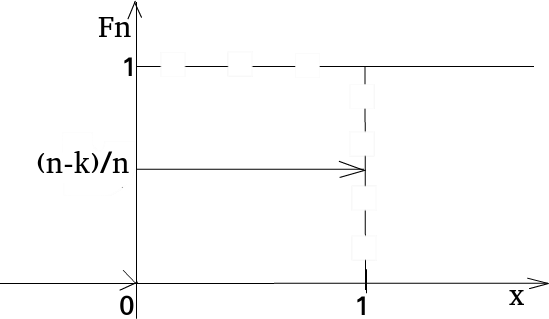
\includegraphics[width=.4\textwidth]{./pictures/1_19.png}
  \caption{Эмпирическая функция распределения}
  \label{fig:119}
\end{figure}

\subsubsection*{1.20}

\textit{Задание.} Пусть $X_1, \dotsc, X_n$ --- выборка из распределения $F$.
Докажите,
что для произвольных $y \in \mathbb{R}$ и $k \in \left\{ 0, 1, \dotsc, n \right\} $
справедливо равенство
$$P \left( F_n \left( y \right) = \frac{k}{n} \right) =
  C_n^k F^k \left( y \right) \left( 1 - F \left( y \right) \right)^{n - k}.$$

\textit{Решение.} Эмпирической функцией распределения, построенной по выборке $X_1, \dotsc, X_n$,
называется функция
$$F_n \left( y \right) =
  \frac{1}{n} \sum \limits_{i = 1}^n \mathbbm{1} \left( X_i \leq y \right).$$

Посмотрим, что значит событие в указанной вероятности
$$F_n \left( y \right) =
  \frac{k}{n} =
  \frac{1}{n} \sum \limits_{i = 1}^n \mathbbm{1} \left( X_i \leq y \right).$$

Сократим константы в знаменателях
$$k =
  \sum \limits_{i = 1}^n \mathbbm{1} \left( X_i \leq y \right).$$
Это означает, что есть ровно $k$ элементов выборки, не превышающих $y$.
Следовательно, это биномиальное распределение с параметром $F \left( y \right) $, то есть
$$P \left( F_n \left( y \right) = \frac{k}{n} \right) =
  C_n^k F^k \left( y \right) \left( 1 - F \left( y \right) \right)^{n - k}.$$

\subsubsection*{1.21}

\textit{Задание.}
Для выборки $X_1, \dotsc, X_n$ из равномерного распределения на отрезке $ \left[ 0, \theta \right] $
найдите плотность, математическое ожидание и дисперсию:
\begin{enumerate}[label=\alph*)]
\item максимального члена вариационного ряда $X_{ \left( n \right) }$;
\item минимального члена вариационного ряда $X_{ \left( 1 \right) }$;
\item совместную плотность распределения и ковариацию $X_{ \left( n \right) }$ и
$X_{ \left( 1 \right) }$.
\end{enumerate}

\textit{Решение.}
\begin{enumerate}[label=\alph*)]
\item Найдём функцию распределения $n$-й порядковой статистики
$F_{X_{ \left( n \right) }} \left( y \right) = \\
  = P \left( X_{ \left( n \right) } \leq y \right) =
  P$ ($n$ элементов выборки не превышают $y$)$=$
  $$= C_n^n \left[ F_{X_1} \left( y \right) \right]^n \cdot
  \left[ 1 - F_{X_1} \left( y \right) \right]^{n - n} =
  \left[ F_{X_1} \left( y \right) \right]^n =
  \left[ P \left( X_1 \leq y \right) \right]^n =
  \left( \frac{y}{ \theta } \right)^n,$$
при этом $y \in \left[ 0, \theta \right] $.

Продифференцируем
$$f_{X_{ \left( n \right) }} \left( y \right) =
  \frac{ \partial F_{X_{ \left( n \right) }} \left( y \right) }{ \partial y} =
  \frac{ \partial }{ \partial y} \left( \frac{y}{ \theta } \right)^n =
  \frac{1}{ \theta^n} \cdot \frac{dy^n}{dy} =
  \frac{ny^{n - 1}}{ \theta^n} \cdot \mathbbm{1} \left\{ y \in \left[ 0, \theta \right] \right\}.$$

По определению математического ожидания
$$MX_{ \left( n \right) } =
  \int \limits_0^{ \theta } ydF^n \left( y \right) =
  \int \limits_0^{ \theta } yd \left( \frac{y}{ \theta } \right)^n =
  \frac{1}{ \theta^n} \int \limits_0^{ \theta } ydy^n =
  \frac{n}{ \theta^n} \int \limits_0^{ \theta } yy^{n - 1} dy.$$
Сложим степени сомножителей
$$ \frac{n}{ \theta^n} \int \limits_0^{ \theta } yy^{n - 1} dy =
  \frac{n}{ \theta^n} \int \limits_0^{ \theta } y^n dy =
  \frac{n}{ \theta^n} \cdot \left. \frac{y^{n + 1}}{n + 1} \right|_0^{ \theta } =
  \frac{ \theta^{n + 1} n}{ \theta^n \left( n + 1 \right) } =
  \frac{ \theta n}{n + 1}.$$

Найдём второй момент
$$MX_{ \left( n \right) }^2 =
  \int \limits_0^{ \theta } y^2 dF^n \left( y \right) =
  \frac{n}{ \theta^n} \int \limits_0^{ \theta } y^2 y^{n - 1} dy =
  \frac{n}{ \theta^n} \int \limits_0^{ \theta } y^{n + 1} dy.$$
Возьмём интеграл
$$ \frac{n}{ \theta^n} \int \limits_0^{ \theta } y^{n + 1} dy =
  \left. \frac{ny^{n + 2}}{ \theta^n \left( n + 2 \right) } \right|_0^{ \theta } =
  \frac{n \theta^{n + 2}}{ \theta^n \left( n + 2 \right) } =
  \frac{n \theta^2}{n + 2}.$$

По свойствам дисперсии
$$DX_{ \left( n \right) } =
  MX_{ \left( n \right) }^2 - \left( MX_{ \left( n \right) } \right)^2 =
  \frac{n \theta^2}{n + 2} - \frac{n^2 \theta^2}{ \left( n + 1 \right)^2}.$$
Приведём к общему знаменателю
\begin{equation*}
  \begin{split}
    \frac{n \theta^2}{n + 2} - \frac{n^2 \theta^2}{ \left( n + 1 \right)^2} =
    \frac{n \theta^2 \left( n^2 + 2n + 1 \right) - n^2 \theta^2 \left( n + 2 \right) }{ \left( n + 2 \right) \left( n + 1 \right)^2} = \\
    = \frac{n^3 \theta^2 + 2n^2 \theta^2 + n \theta^2 - n^3 \theta^2 - 2n^2 \theta^2}{ \left( n + 2 \right) \left( n + 1 \right)^2} =
    \frac{n \theta^2}{ \left( n + 2 \right) \left( n + 1 \right)^2};
  \end{split}
\end{equation*}
\item найдём функцию распределения первой порядковой статистики
$$F_{X_{ \left( 1 \right) }} \left( y \right) =
  P \left( X_{ \left( 1 \right) } \leq y \right) =
  P \left( \min \left( X_1, X_2, \dotsc, X_n \right) \leq y \right) =$$
  $= P$(хотя бы 1 элемент выборки не превышает $y$)$ =$
\begin{equation*}
  \begin{split}
    \sum \limits_{k = 1}^n
    P \left(exactly \, k \, elements \, of \, the \, sample \, does \, not \, exceed \, y \right) = \\
    = \sum \limits_{k = 1}^n C_n^k F^k \left( y \right) \left[ 1 - F \left( y \right) \right]^{n - k} = \\
    = \sum \limits_{k = 0}^n
      C_n^k F^k \left( y \right) \left[ 1 - F \left( y \right) \right]^{n - k} -
    C_n^0 F^0 \left( y \right) \left[ 1 - F \left( y \right) \right]^{n - 0}.
  \end{split}
\end{equation*}
Применяем формулу для бинома Ньютона
\begin{equation*}
  \begin{split}
    \sum \limits_{k = 0}^n
    C_n^k F^k \left( y \right) \left[ 1 - F \left( y \right) \right]^{n - k} -
    C_n^0 F^0 \left( y \right) \left[ 1 - F \left( y \right) \right]^{n - 0} = \\
    = \left[ F \left( y \right) + 1 - F \left( y \right) \right]^n -
    \left[ 1 - F \left( y \right) \right]^n =
    1 - \left( 1 - \frac{y}{ \theta } \right)^n.
  \end{split}
\end{equation*}

Продифференцируем
$$f_{X_{ \left( 1 \right) }} \left( y \right) =
  \frac{ \partial F_{X_{ \left( 1 \right) }} \left( y \right) }{ \partial y} =
  \frac{ \partial }{ \partial y}
    \left( 1 - \frac{ \left( \theta - y \right)^n}{ \theta^n} \right) =
  - \frac{1}{ \theta^n} \cdot \frac{ \partial }{ \partial y} \left( \theta - y \right)^n.$$
Берём производную сложной функции
$$- \frac{1}{ \theta^n} \cdot \frac{ \partial }{ \partial y} \left( \theta - y \right)^n
  - \frac{1}{ \theta^n} \cdot n \left( \theta - y \right)^{n - 1} \left( -1 \right) =
  \frac{n \left( \theta - y \right)^{n - 1}}{ \theta^n}, \,
  y \in \left[ 0, \theta \right].$$

Найдём математическое ожидание по определению
$$MX_{ \left( 1 \right) } =
  \int \limits_0^{ \theta } ydF^n \left( y \right) =
  \int \limits_0^{ \theta } yd \left( 1 - \frac{y}{ \theta } \right)^n.$$
Сделаем замену
$$1 - \frac{y}{ \theta } =
  z,$$
откуда $y = \theta \left( 1 - z \right) $,
при этом интегрирование происходит в пределах от одного до нуля
$$ \int \limits_0^{ \theta } yd \left( 1 - \frac{y}{ \theta } \right)^n =
  \int \limits_1^0 \theta \left( 1 - z \right) dz^n =
  \theta n \int \limits_1^0 \left( z - 1 \right) z^{n - 1} dz.$$
Разбиваем на 2 интеграла
$$ \theta n \int \limits_1^0 \left( z - 1 \right) z^{n - 1} dz =
  - \theta n \int \limits_0^1 z^n dz + \theta n \int \limits_0^1 z^{n - 1} dz =
  - \theta n \cdot \left. \frac{z^{n + 1}}{n + 1} \right|_0^1 +
  \theta n \cdot \left. \frac{z^n}{n} \right|_0^1.$$
Подставляем пределы интегрирования
$$- \theta n \cdot \left. \frac{z^{n + 1}}{n + 1} \right|_0^1 +
  \theta n \cdot \left. \frac{z^n}{n} \right|_0^1 =
  - \theta n \cdot \frac{1}{n + 1} + \theta n \cdot \frac{1}{n} =
  - \theta n \left( \frac{1}{n + 1} - \frac{1}{n} \right).$$
Приводим к общему знаменателю
$$ - \theta n \left( \frac{1}{n + 1} - \frac{1}{n} \right) =
  - \theta n \cdot \frac{n - n - 1}{n \left( n + 1 \right) } =
  \frac{ \theta n}{n \left( n + 1 \right) } =
  \frac{ \theta }{ \left( n + 1 \right) }.$$

Найдём второй момент
$$MX_{ \left( 1 \right) }^2 =
  \int \limits_0^{ \theta } y^2 d \left( 1 - \frac{y}{ \theta } \right)^n.$$
Применяем такую же замену, как при поиске первого момента
$$ \int \limits_0^{ \theta } y^2 d \left( 1 - \frac{y}{ \theta } \right)^n =
  \int_1^0 \theta^2 \left( 1 - z \right)^2 dz^n =
  \int_0^1 \theta^2 n \left( 1 - z \right)^2 z^{n - 1} dz.$$
Выносим константу за знак интеграла и возводим скобку в квадрат
\begin{equation*}
  \begin{split}
    \int_0^1 \theta^2 n \left( 1 - z \right)^2 z^{n - 1} dz =
    \theta^2 n \int \limits_0^1 \left( 1 - 2z + z^2 \right) z^{n - 1} dz = \\
    = \theta^2 n \int \limits_0^1 z^{n - 1} dz -
    2 \theta^2 n \int \limits_0^1 z^n dz +
    \theta^2 n \int \limits_0^1 z^{n + 1} dz = \\
    = \theta^2 n \cdot \left. \frac{z^n}{n} \right|_0^1 -
    2 \theta^2 n \cdot \left. \frac{z^{n + 1}}{n + 1} \right|_0^1 +
    \theta^2 n \cdot \left. \frac{z^{n + 2}}{n + 2} \right|_0^1 =
    \theta^2 - \frac{2 \theta^2 n}{n + 1} + \frac{ \theta^2 n}{n + 2} = \\
    = \theta^2 \left( 1 - \frac{2n}{n + 1} + \frac{n}{n + 2} \right) = \\
    = \theta^2 \cdot
    \frac{ \left( n + 1 \right) \left( n + 2 \right) - 2n \left( n + 2 \right) + n \left( n + 1 \right) }{ \left( n + 1 \right) \left( n + 2 \right) } = \\
    = \frac{ \theta^2 \left( n^2 + 3n + 2 - 2n^2 - 4n + n^2 + n \right) }{ \left( n + 1 \right) \left( n + 2 \right) } =
    \frac{2 \theta^2}{ \left( n + 1 \right) \left( n + 2 \right) }.
  \end{split}
\end{equation*}

По свойствам дисперсии
$$DX_{ \left( 1 \right) } =
  MX_{ \left( 1 \right) }^2 - \left[ MX_{ \left( 1 \right) } \right]^2 =
  \frac{2 \theta^2}{ \left( n + 1 \right) \left( n + 2 \right) } -
  \frac{ \theta^2}{ \left( n + 1 \right)^2}.$$
Приводим к общему знаменателю
\begin{equation*}
  \begin{split}
    \frac{2 \theta^2}{ \left( n + 1 \right) \left( n + 2 \right) } -
    \frac{ \theta^2}{ \left( n + 1 \right)^2} =
    \frac{2 \theta^2 \left( n + 1 \right) - \theta^2 \left( n + 2 \right) }{ \left( n + 1 \right)^2 \left( n + 2 \right) } = \\
    = \frac{2 \theta^2 n + 2 \theta^2 - \theta^2 n - 2 \theta^2}{ \left( n + 1 \right)^2 \left( n + 2 \right) } =
    \frac{ \theta^2 n}{ \left( n + 1 \right)^2 \left( n + 2 \right) };
  \end{split}
\end{equation*}
\item найдём функцию распределения вектора по определению
$$F_{ \left( X_{ \left( 1 \right)}, X_{ \left( n \right) } \right) } \left( y_1, y_n \right)=
  P \left( X_{ \left( 1 \right) } \leq y_1, X_{ \left( n \right) } \leq y_n \right).$$
Воспользовавшись формулой
$P \left( A \cap B \right) =
  P \left( B \right) - P \left( \overline{A} \cap B \right) $,
получим
$$P \left( X_{ \left( 1 \right) } \leq y_1, X_{ \left( n \right) } \leq y_n \right) =
    P \left( X_{ \left( n \right) } \leq y_n \right) -
    P \left( X_{ \left( 1 \right) } > y_1, \, X_{ \left( n \right) } \leq y_n \right).$$
Если максимум меньше какого-то значения, то все элементы меньше него
\begin{equation*}
  \begin{split}
    P \left( X_{ \left( 1 \right) } > y_1, \, X_{ \left( n \right) } \leq y_n \right) = \\
    = P \left( X_1 \leq y_n, \dotsc, X_n \leq y_n \right) - \\
    = P \left(
      X_1 \in \left( y_1, y_n \right], \,
      X_2 \in \left( y_1, y_n \right],
      \dotsc,
      X_n \in \left( y_1, y_n \right]
    \right) = \\
    = \left[ F \left( y_n \right) \right]^n -
    \left[ F \left( y_n \right) - F \left( y_1 \right) \right]^n
  \end{split}
\end{equation*}
при $y_1 < y_n$.

Продифференцируем
\begin{equation*}
  \begin{split}
    f_{ \left( X_{ \left( 1 \right) }, X_{ \left( n \right) } \right) } \left( y_1, y_n \right) =
    \begin{cases}
      0, \qquad y_1 \geq y_n, \\
      n \left( n - 1 \right) \cdot
      \left[ F \left( y_n \right) - F \left( y_1 \right) \right]^{n - 2} \times \\
      \times p_{X_1} \left( y_1 \right) p_{X_n} \left( y_n \right) = \\
      = n \left( n - 1 \right) \cdot
      \left[ \frac{y_n}{ \theta } - \frac{y_1}{ \theta } \right]^{n - 2} \cdot
      \frac{1}{ \theta^2} = \\
      = n \left( n - 1 \right) \cdot \frac{ \left( y_n - y_1 \right)^n}{ \theta^{n - 2}} \cdot
      \frac{1}{ \theta^2} =
      \frac{n \left( n - 1 \right) \left( y_n - y_1 \right)^{n - 1}}{ \theta^n}.
    \end{cases}
  \end{split}
\end{equation*}

Найдём математическое ожидание вектора
$$M \left( X_{ \left( 1 \right) }, X_{ \left( n \right) } \right) =
    \frac{n \left( n - 1 \right) }{ \theta^n} \cdot
    \int \limits_0^{ \theta }
      \int \limits_{y_n}^{ \theta } y_1 y_n \left( y_n - y_1 \right)^{n - 2} dy_1
    dy_n.$$

Заменим разность величин величиной $x$.
Якобиан преобразования равен
$$ \frac{ \partial \left( x, y_n \right) }{ \partial \left( x, y_1 \right) } =
  \left|
    \begin{bmatrix}
      \frac{ \partial x}{ \partial y_1} & \frac{ \partial y_n}{ \partial y_1} \\
      \frac{ \partial x}{ \partial y_n} & \frac{ \partial y_1}{ \partial y_1}
    \end{bmatrix}
  \right| =
  \left|
    \begin{bmatrix}
      1 & 0 \\
      -1 & 1
    \end{bmatrix}
  \right| =
  1.$$
Получаем
\begin{equation*}
  \begin{split}
    \frac{n \left( n - 1 \right) }{ \theta^n} \cdot
    \int \limits_0^{ \theta }
      \int \limits_{y_n}^{ \theta } y_1 y_n \left( y_n - y_1 \right)^{n - 2} dy_1
    dy_n = \\
    = \frac{n \left( n - 1 \right) }{ \theta^n} \cdot
    \int \limits_0^{ \theta }
      \int \limits_0^{ \theta - y_n} \left( x + y_n \right) y_n x^{n - 2} dx
    dy_n = \\
    = \frac{n \left( n - 1 \right) }{ \theta^n} \cdot
    \int \limits_0^{ \theta } y_n dy_n \cdot
      \int \limits_0^{ \theta - y_n} \left( x^{n - 1} + y_n x^{n - 2} \right) dx = \\
    = \frac{n \left( n - 1 \right) }{ \theta^n} \cdot
    \int \limits_0^{ \theta } y_n dy_n \cdot
      \left.
        \left( \frac{x^n}{n} + y_n \cdot \frac{x^{n - 1}}{n - 1} \right)
      \right|_0^{ \theta - y_n} = \\
    = \frac{1}{ \theta^n}  \cdot
    \int \limits_0^{ \theta }
      \left[
        \left( n - 1 \right) \left( \theta - y_n \right) + y_n n \left( \theta - y_n \right)^{n - 1}
      \right] \cdot
      y_n
    dy_n = \\
    = \frac{1}{ \theta^n} \cdot
    \int \limits_0^{ \theta }
      \left( \theta - y_n \right)^{n - 1} \cdot
      \left[ \left( n - 1 \right) \left( \theta - y_n \right) + y_n n \right] \cdot
      y_n
    dy_n = \\
    = \frac{1}{ \theta^n} \cdot
    \int \limits_0^{ \theta }
      \left( \theta - y_n \right)^{n - 1} \left[ n \theta - \left( \theta - y_n \right) \right] y_n
    dy_n.
  \end{split}
\end{equation*}
Заменяем первую скобку в интеграле на $t$.
Получаем
$$ \frac{1}{ \theta^n} \cdot
  \int \limits_0^{ \theta }
    \left( \theta - y_n \right)^{n - 1} \left[ n \theta - \left( \theta - y_n \right) \right] y_n
  dy_n =
  \frac{1}{ \theta^n} \cdot
  \int \limits_0^{ \theta } t^{n - 1} \left( n \theta - t \right) \left( \theta - t \right) dt.$$
Перемножаем скобки
\begin{equation*}
  \begin{split}
    \frac{1}{ \theta^n} \cdot
    \int \limits_0^{ \theta } t^{n - 1} \left( n \theta - t \right) \left( \theta - t \right) dt =
    \frac{1}{ \theta^n} \cdot
    \int \limits_0^{ \theta }
      t^{n - 1} \left( n \theta^2 - \left( n + 1 \right) \theta t + t^2 \right)
    dt = \\
    = \frac{1}{ \theta^n} \cdot
    \int \limits_0^{ \theta }
      \left( n \theta^2 t^{n - 1} - \left( n + 1 \right) \theta t^n + t^{n + 1} \right)
    dt = \\
    = \frac{1}{ \theta^n} \cdot
    \left.
      \left[ \theta^2 t^n - \theta t^{n + 1} + \frac{t^{n + 2}}{n + 2} \right]
    \right|_0^{ \theta } =
    \frac{1}{ \theta^n} \cdot
    \left[ \theta^{n + 2} - \theta^{n + 2} + \frac{ \theta^{n + 2}}{n + 2} \right] =
    \frac{ \theta^2}{n + 2}.
  \end{split}
\end{equation*}

По определению ковариации
$$cov \left( X_{ \left( 1 \right) }, X_{ \left( n \right) } \right) =
  M \left( X_{ \left( 1 \right) } X_{ \left( n \right) } \right) -
  MX_{ \left( 1 \right) } MX_{ \left( n \right) } =
  \frac{ \theta^2}{n + 2} - \frac{ \theta }{n + 1} \cdot \frac{ \theta n}{n + 1}.$$
Выносим общий множитель за скобки
$$ \frac{ \theta^2}{n + 2} - \frac{ \theta }{n + 1} \cdot \frac{ \theta n}{n + 1} =
  \theta^2 \left( \frac{1}{n + 2} - \frac{n}{ \left( n + 1 \right)^2} \right).$$
Приводим к общему знаменателю дроби в скобках
$$ \theta^2 \left( \frac{1}{n + 2} - \frac{n}{ \left( n + 1 \right)^2} \right) =
  \theta^2 \cdot \frac{n^2 + 2n + 1 - n^2 - 2n}{ \left( n + 2 \right) \left( n + 1 \right)^2} =
  \frac{ \theta^2}{ \left( n + 2 \right) \left( n + 1 \right)^2}.$$
\end{enumerate}

\subsubsection*{1.22}

\textit{Задание.}
Пусть задана выборка $X_1, \dotsc, X_n$ из показательного распределения с параметром $ \alpha $.
Докажите, что
$$MX_{ \left( k \right) } =
  \frac{1}{ \alpha } \left( \frac{1}{n - k + 1} + \dotsc + \frac{1}{n} \right),$$
не находя распределения порядковой статистики $X_{ \left( k \right) }$.

\textit{Решение.} Преобразуем левую часть того, что нужно доказать
$$MX_{ \left( k \right) } =
  MX_{ \left( 1 \right) } +
  \sum \limits_{i = 1}^{k - 1}
    M \left( X_{ \left( i + 1 \right) } - X_{ \left(i \right) } \right).$$

Элементы выборки имеют плотность распределения
$$p \left( y \right) =
  \alpha e^{- \alpha y} \cdot \mathbbm{1} \left\{ y \geq 0 \right\}.$$

Интегрируя плотность, получим функцию распределения
$$F \left( y \right) =
  \int \limits_{- \infty }^y p \left( x \right) dx =
  \int \limits_{- \infty }^y \alpha e^{- \alpha x} \cdot \mathbbm{1} \left\{ x \geq 0 \right\} dx =
  \int \limits_0^y \alpha e^{- \alpha x} dx =
  \left. -e^{- \alpha x} \right|_0^y.$$
Подставляем пределы интегрирования
$$ \left. -e^{- \alpha x} \right|_0^y =
  1 - e^{- \alpha y}, \,
  y \geq 0.$$

Находим функцию распределения минимальной порядковой статистики
$$F_{X_{ \left( 1 \right) }} \left( y \right) =
  P \left( X_{ \left( 1 \right) } \leq y \right) =
  1 - P \left( X_{ \left( 1 \right) } > y \right).$$
Если минимальный элемент выборки больше какого-то значения, то все элементы выборки больше него
$$1 - P \left( X_{ \left( 1 \right) } > y \right) =
  1 - P \left( X_1 > y, X_2 > y, \dotsc, X_n > y \right).$$
Из независимости случайных величин следует, что
$$1 - P \left( X_1 > y, X_2 > y, \dotsc, X_n > y \right) =
  1 -
  P \left( X_1 > y \right) \cdot
  P \left( X_2 > y \right) \cdot
  \dotsc \cdot
  P \left( X_n > y \right).$$
Переходим к противоположным событиям и учитываем то, что случайные величины одинаково распределены
$$1 -
  P \left( X_1 > y \right) \cdot
  P \left( X_2 > y \right) \cdot
  \dotsc \cdot
  P \left( X_n > y \right) =
  1 - \left[ 1 - F \left( y \right) \right]^n.$$

Находим плотность минимальной порядковой статистики
$$f_{X_{ \left( 1 \right) }} \left( y \right) =
  \frac{ \partial F_{X_{ \left( 1 \right) }} \left( y \right) }{ \partial y} =
  \frac{ \partial \left\{ 1 - \left[ 1 - F \left( y \right) \right]^n \right\} }{ \partial y} =
  -n \left[ 1 - F \left( y \right) \right]^{n - 1} \cdot \left( -1 \right) f \left( y \right).$$
Упрощаем и учитываем, что $f \left( y \right) $ --- это плотность распределения элементов выборки
$$-n \left[ 1 - F \left( y \right) \right]^{n - 1} \cdot \left( -1 \right) f \left( y \right) =
  n \left[ 1 - F \left( y \right) \right]^{n - 1} p \left( y \right).$$
Подставляем функцию и плотность распределения
$$n \left[ 1 - F \left( y \right) \right]^{n - 1} p \left( y \right) =
  n \left[ 1 - \left( 1 - e^{- \alpha y} \right) \right]^n \alpha e^{- \alpha y} \cdot
  \mathbbm{1} \left\{ y \geq 0 \right\}.$$
Упрощаем выражение в скобках
$$n \left[ 1 - \left( 1 - e^{- \alpha y} \right) \right]^n \alpha e^{- \alpha y} \cdot
  \mathbbm{1} \left\{ y \geq 0 \right\} =
  n \alpha e^{- \alpha \left( n - 1 \right) y} e^{- \alpha y} \cdot
  \mathbbm{1} \left\{ y \geq 0 \right\}.$$
Суммируем показатели экспонент
$$n \alpha e^{- \alpha \left( n - 1 \right) y} e^{- \alpha y} \cdot
  \mathbbm{1} \left\{ y \geq 0 \right\} =
  n \alpha e^{- \alpha ny} \cdot \mathbbm{1} \left\{ y \geq 0 \right\}.$$
Отсюда следует, что $X_{ \left( 1 \right) } \sim Exp \left( n \alpha \right) $.

Из задачи 1.11 б)
$X_{ \left( i + 1 \right) } - X_{ \left( i \right) } \sim
  Exp \left( \alpha \left( n - i \right) \right) $.

Тогда такая разность имеет математическое ожидание
$$M \left( X_{ \left( i + 1 \right) } - X_{ \left( i \right) } \right) =
  \frac{1}{ \alpha \left( n - i \right) }.$$

Подставялем в полученное в начале выражение
$$MX_{ \left( 1 \right) } +
  \sum \limits_{i = 1}^{k - 1}
    M \left( X_{ \left( i + 1 \right) } - X_{ \left(i \right) } \right) =
  \frac{1}{n \alpha } + \sum \limits_{i = 1}^{k - 1} \frac{1}{ \alpha \left( n - i \right) }.$$
Записываем сумму в явном виде
$$ \frac{1}{n \alpha } + \sum \limits_{i = 1}^{k - 1} \frac{1}{ \alpha \left( n - i \right) } =
  \frac{1}{ \alpha } \cdot
  \left( \frac{1}{n} + \frac{1}{n - 1} + \frac{1}{n - 2} + \dotsc + \frac{1}{n - k + 1} \right).$$
